\chapter{Conclusiones}

\section{Presentación de Resultados}

\begin{figure}[h!]
    \centering
    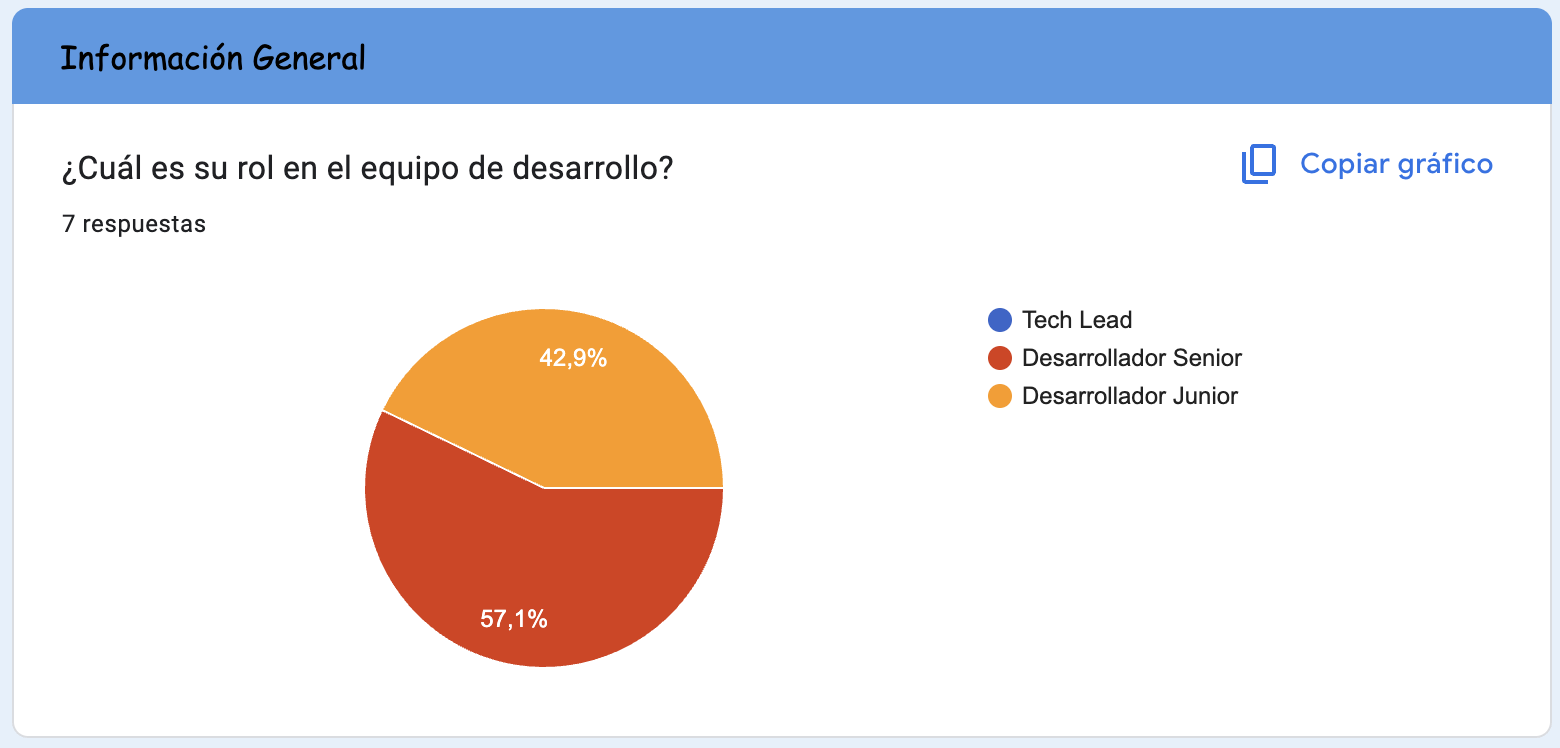
\includegraphics[width=1\textwidth]{images/question_1.png}
    \caption{Encuesta: Pregunta 1}
    \label{fig:question_1}
\end{figure}

\FloatBarrier

Esto indica que un 57 \% es desarrollador Senior, lo cual refleja que esta encuesta estará predominada por personas con bastante experiencia en el rubro de la industria del software.

\FloatBarrier
\begin{figure}[h!]
    \centering
    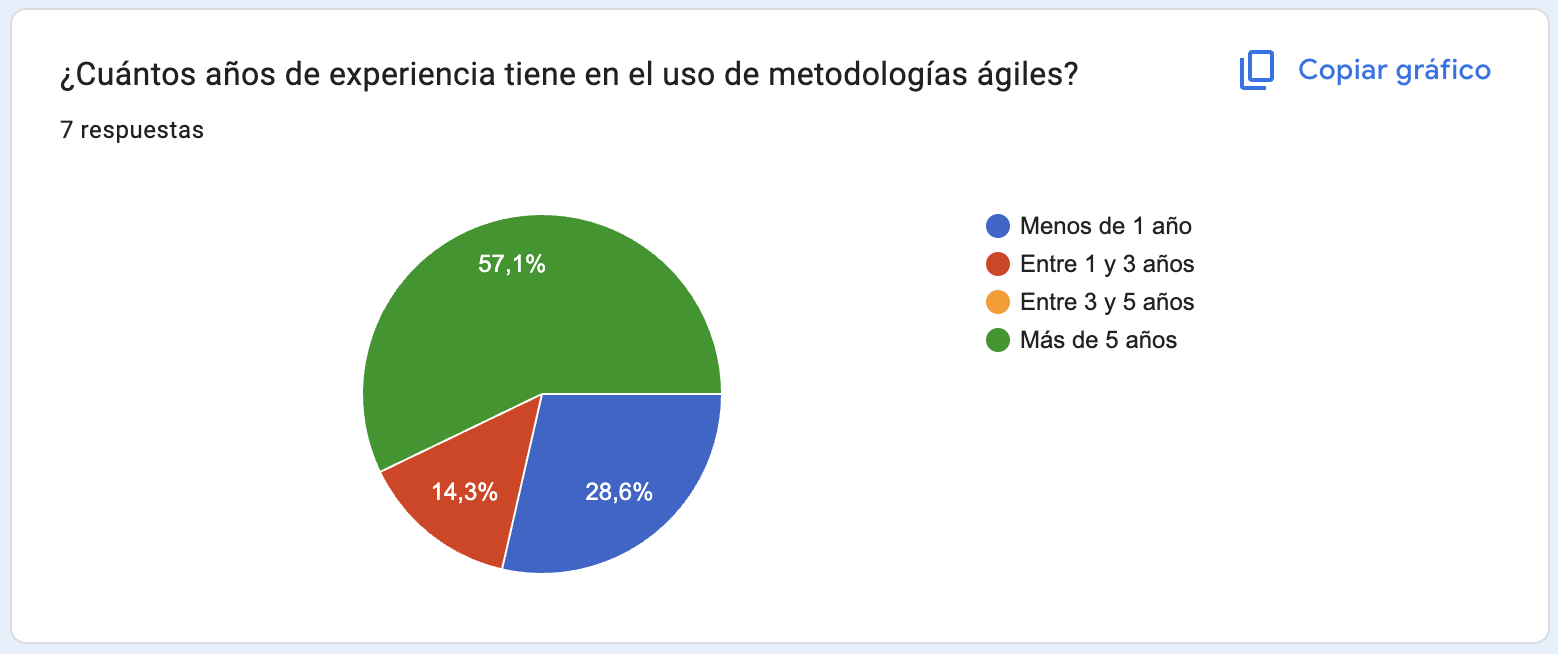
\includegraphics[width=1\textwidth]{images/question_2.png}
    \caption{Encuesta: Pregunta 2}
    \label{fig:question_2}
\end{figure}

\FloatBarrier
Esta imagen nos indica que el 57.1\% ya ha trabajado con alguna metología ágil, es decir que en sus equipos de trabajo es casi un estilo de trabajo en equipo usando estas metodologías, lo que podría reflejar que no sería difícil poder ajustarse a las empresas a ajustarse usando el mismo modelo de estimaciones, pero aplicado en los costos.


\FloatBarrier
\begin{figure}[h!]
    \centering
    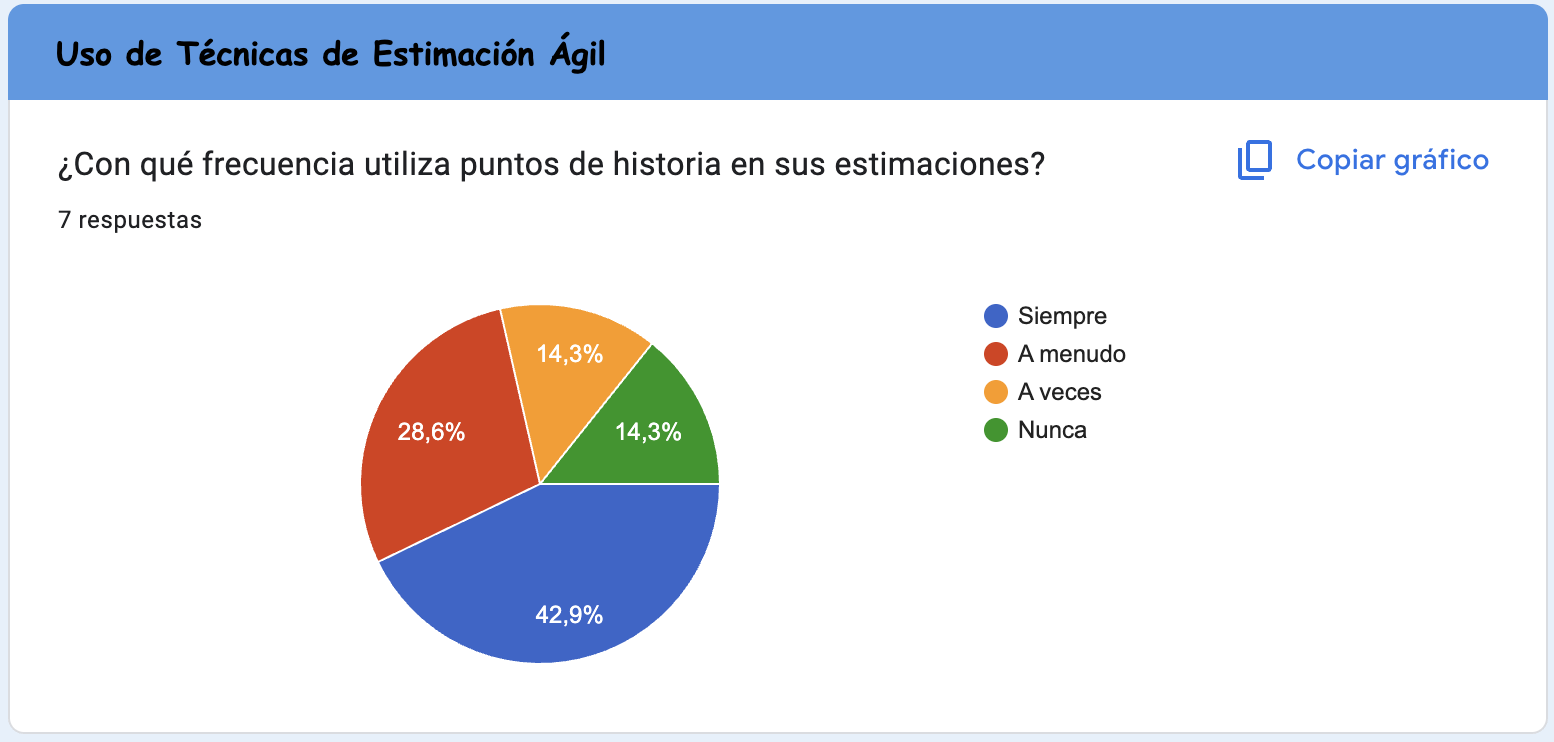
\includegraphics[width=1\textwidth]{images/question_3.png}
    \caption{Encuesta: Pregunta 3}
    \label{fig:question_3}
\end{figure}

\FloatBarrier
Este comportamiento refleja que, aunque los puntos de historia son ampliamente aceptados como una técnica ágil efectiva, existe un porcentaje considerable de equipos que no los utilizan con regularidad. Las razones pueden deberse a la falta de experiencia con metodologías ágiles, el tamaño reducido de los equipos, o la percepción de que la técnica no aporta valor en ciertos contextos específicos. Es importante analizar las barreras que limitan su adopción para proponer estrategias que promuevan su uso consistente y efectivo.

\FloatBarrier
\begin{figure}[h!]
    \centering
    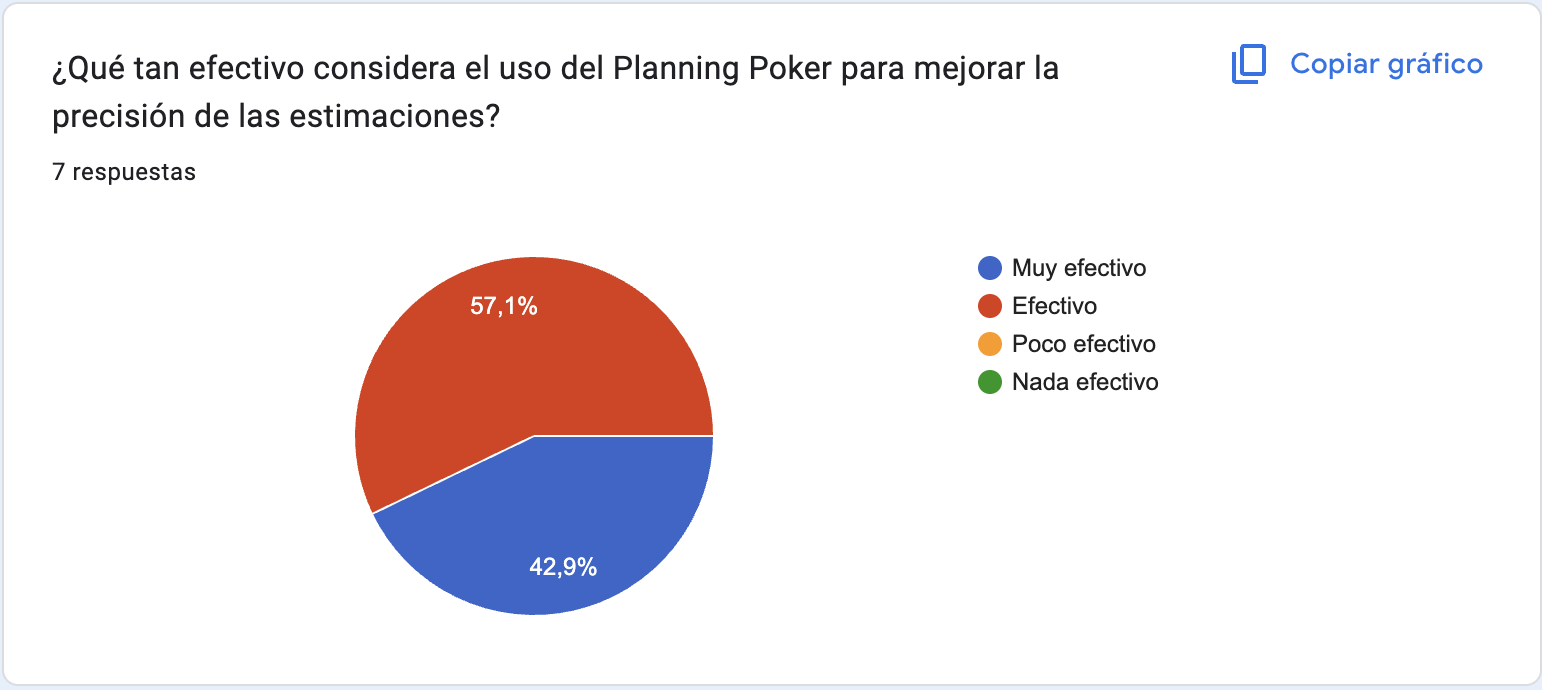
\includegraphics[width=1\textwidth]{images/question_4.png}
    \caption{Encuesta: Pregunta 4}
    \label{fig:question_4}
\end{figure}


\FloatBarrier
El gráfico ilustra la percepción de los encuestados sobre la efectividad del Planning Poker para mejorar la precisión en las estimaciones. Se observa que el 57.1\% considera esta técnica como efectiva, mientras que un 42.9\% la califica como muy efectiva.

Estos resultados reflejan un alto nivel de aceptación de Planning Poker dentro de los equipos de desarrollo, confirmando su utilidad como herramienta colaborativa para alcanzar estimaciones más precisas. La participación activa de los miembros del equipo en el proceso fomenta el consenso y permite ajustar las percepciones individuales, reduciendo la incertidumbre y mejorando la calidad de las proyecciones. Sin embargo, la ausencia de respuestas negativas (poco efectivo o nada efectivo) indica que, en los equipos evaluados, Planning Poker se ha consolidado como una práctica eficiente y valorada en contextos ágiles.

\FloatBarrier
\begin{figure}[h!]
    \centering
    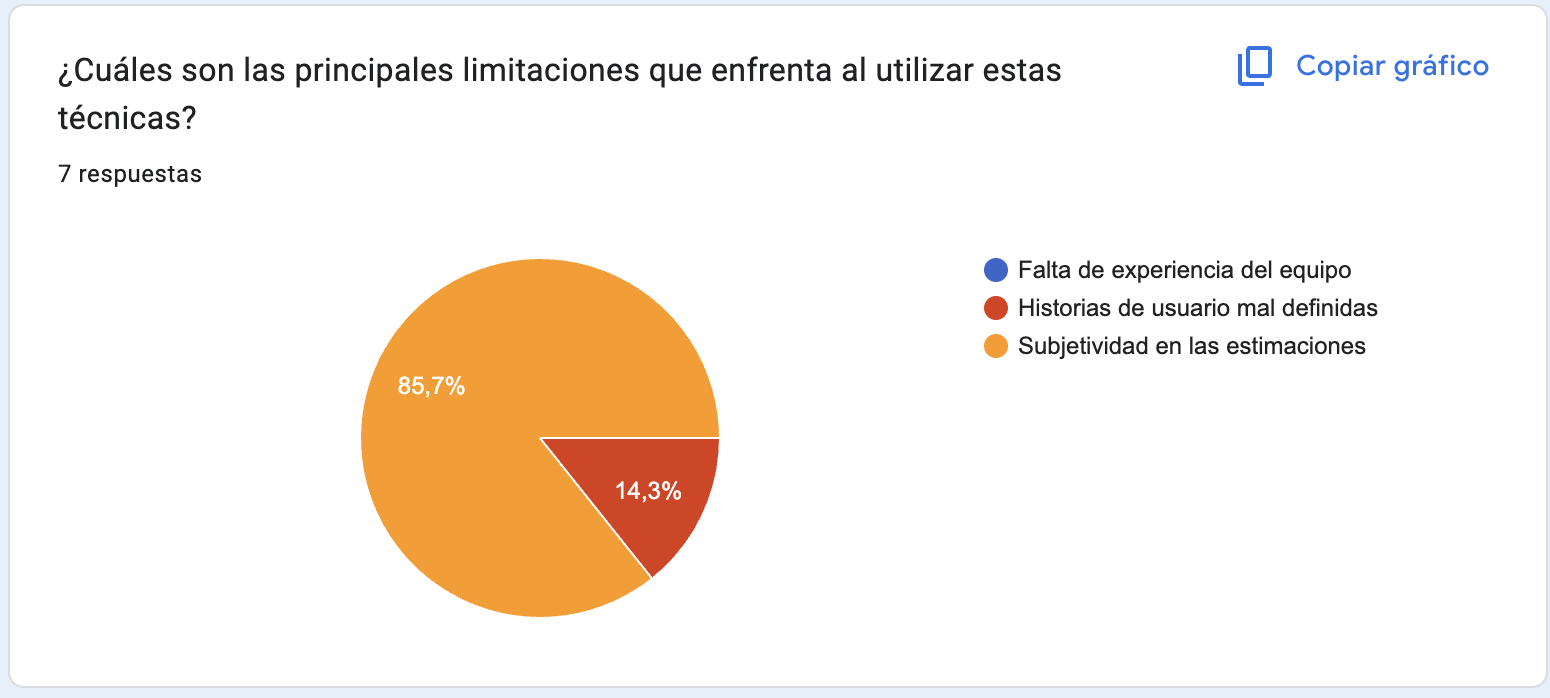
\includegraphics[width=1\textwidth]{images/question_5.png}
    \caption{Encuesta: Pregunta 5}
    \label{fig:question_5}
\end{figure}


\FloatBarrier
Es relevante destacar que no se mencionó la falta de experiencia del equipo como una limitación, lo cual sugiere que los participantes cuentan con un nivel adecuado de conocimiento en metodologías ágiles. Sin embargo, los resultados subrayan la necesidad de implementar prácticas que reduzcan la subjetividad en las estimaciones, como el uso de datos históricos, métricas más objetivas y un mejor refinamiento de las historias de usuario.

\section{Conclusiones Generales}
El presente análisis sobre la estimación de costos en el desarrollo de software utilizando enfoques ágiles, como los puntos de historia y el Planning Poker, permite identificar tanto la aceptación como los desafíos asociados a estas técnicas dentro de los equipos de desarrollo.

En primer lugar, los resultados muestran que un 42.9\% de los encuestados utiliza los puntos de historia de manera constante, lo que refleja una alta adopción de esta herramienta como método principal de estimación en equipos ágiles. Sin embargo, un 28.6\% lo usa con menos frecuencia, lo que podría indicar variabilidad en su implementación dependiendo del contexto o de la experiencia del equipo.

En relación con el Planning Poker, la técnica es percibida positivamente, con un 57.1\% calificándola como efectiva y un 42.9\% como muy efectiva. Esta evaluación confirma la utilidad de Planning Poker como una herramienta colaborativa para mejorar la precisión de las estimaciones, especialmente al fomentar la participación del equipo y alcanzar consensos.

Por otro lado, se evidencian limitaciones importantes en el uso de estas técnicas. La subjetividad en las estimaciones fue identificada como el principal desafío por el 85.7\% de los encuestados, lo que subraya la necesidad de minimizar la variabilidad mediante mejores prácticas y herramientas complementarias. Adicionalmente, un 14.3\% señaló las historias de usuario mal definidas como una barrera significativa, lo que destaca la importancia de contar con requerimientos claros y bien estructurados para obtener estimaciones más precisas.

En conclusión, aunque las técnicas de puntos de historia y Planning Poker son valoradas positivamente y ampliamente adoptadas, su efectividad depende en gran medida de factores como la claridad de los requerimientos, la experiencia del equipo y la implementación de mecanismos que reduzcan la subjetividad. Es necesario fomentar un proceso más riguroso de definición de historias de usuario y explorar el uso de datos históricos o herramientas de análisis predictivo para mejorar la objetividad y consistencia de las estimaciones en proyectos ágiles de desarrollo de software.